\documentclass[10pt]{article}
\usepackage[margin=.78in]{geometry}
\usepackage[T1]{fontenc}
\usepackage{lmodern,microtype,booktabs,tabularx,graphicx,hyperref,xcolor}
\emergencystretch=3em
\title{Final Phase 3 Research Improvement\\External Evaluation and Calibration Failure Analysis}
\author{Umar Behram (23I-2604) \and Ahmed Bilal (23I-2581)}
\date{Day 3 final research-improvement edition -- 15 November 2026}
\begin{document}
\maketitle
\begin{abstract}
This final package preserves the submitted Phase 2 basis and all earlier snapshots, then adds one UCI external cohort evaluation and a pre-specified-after-primary exploratory diagnosis. The corrected 60/20/20 history split uses only 267/89/89 rows from UCI batch 1; whole batches 2-10 are evaluated without invented within-batch times. Across nine cohorts, mean accuracy is 0.432, fixed-six-class macro-F1 is 0.290, and the frozen confidence-based accuracy estimator has MAE 0.545. Its approximate plug-in intervals cover 0/9 cohort accuracies. Exploratory class-mix standardization does not remove the degradation, and source confidence overstates cohort correctness by 0.18-0.57. These findings support a dataset-specific calibration-transfer failure, not generalization claims.
\end{abstract}

\section{What changed and why}
Day 1 packaged and validated the existing controlled synthetic evidence. Day 2 admitted UCI dataset 224 after checking source terms, ten cohort files, class coverage, feature validity, duplicates, and source hash. The first implementation allocated its history split incorrectly; its run and raw outputs are retained under the explicitly superseded v1 path. The corrected v2 runner follows the previously locked 60/20/20 split and records exact row indices. Day 3 asked, before computing its new diagnostic, whether class composition accounts for the external performance decline and whether source confidence transfers. No model or threshold was retuned.

\section{External evaluation}
The UCI source comprises 13,910 measurements, 128 features, six classes and ten acquisition batches \cite{uci224}. Batch 1 contains 445 rows; it supplies 267 training, 89 calibration and 89 reference examples by fixed stratified splits. Whole future batches have sizes 161-3,613, with changing class proportions and some missing classes. The source page shows a CC BY 4.0 license but also describes the data as research-only and excludes commercial use; this project follows the more restrictive description.

The standardized multinomial logistic classifier and three-component PCA were fitted only on training rows. A fixed logistic calibration map from maximum class probability to correctness used only the separate calibration rows. Per-cohort input alarms use Holm-corrected KS tests over 128 original features and three frozen PCA coordinates. Accuracy intervals use a continuity-corrected normal approximation to a plug-in Poisson-binomial distribution. They assume independent correctness probabilities and ignore calibration uncertainty.

Across the nine held-out cohorts, mean observed accuracy is 0.432, fixed-label macro-F1 is 0.290, mean estimated accuracy is 0.976, and mean absolute estimation error is 0.545. All nine batches trigger at least one input alarm. Approximate interval coverage is 0/9, with mean width 0.026. This is a descriptive cohort count from one dataset, not a population coverage guarantee or known-onset recall result.

\begin{figure}[h]
\centering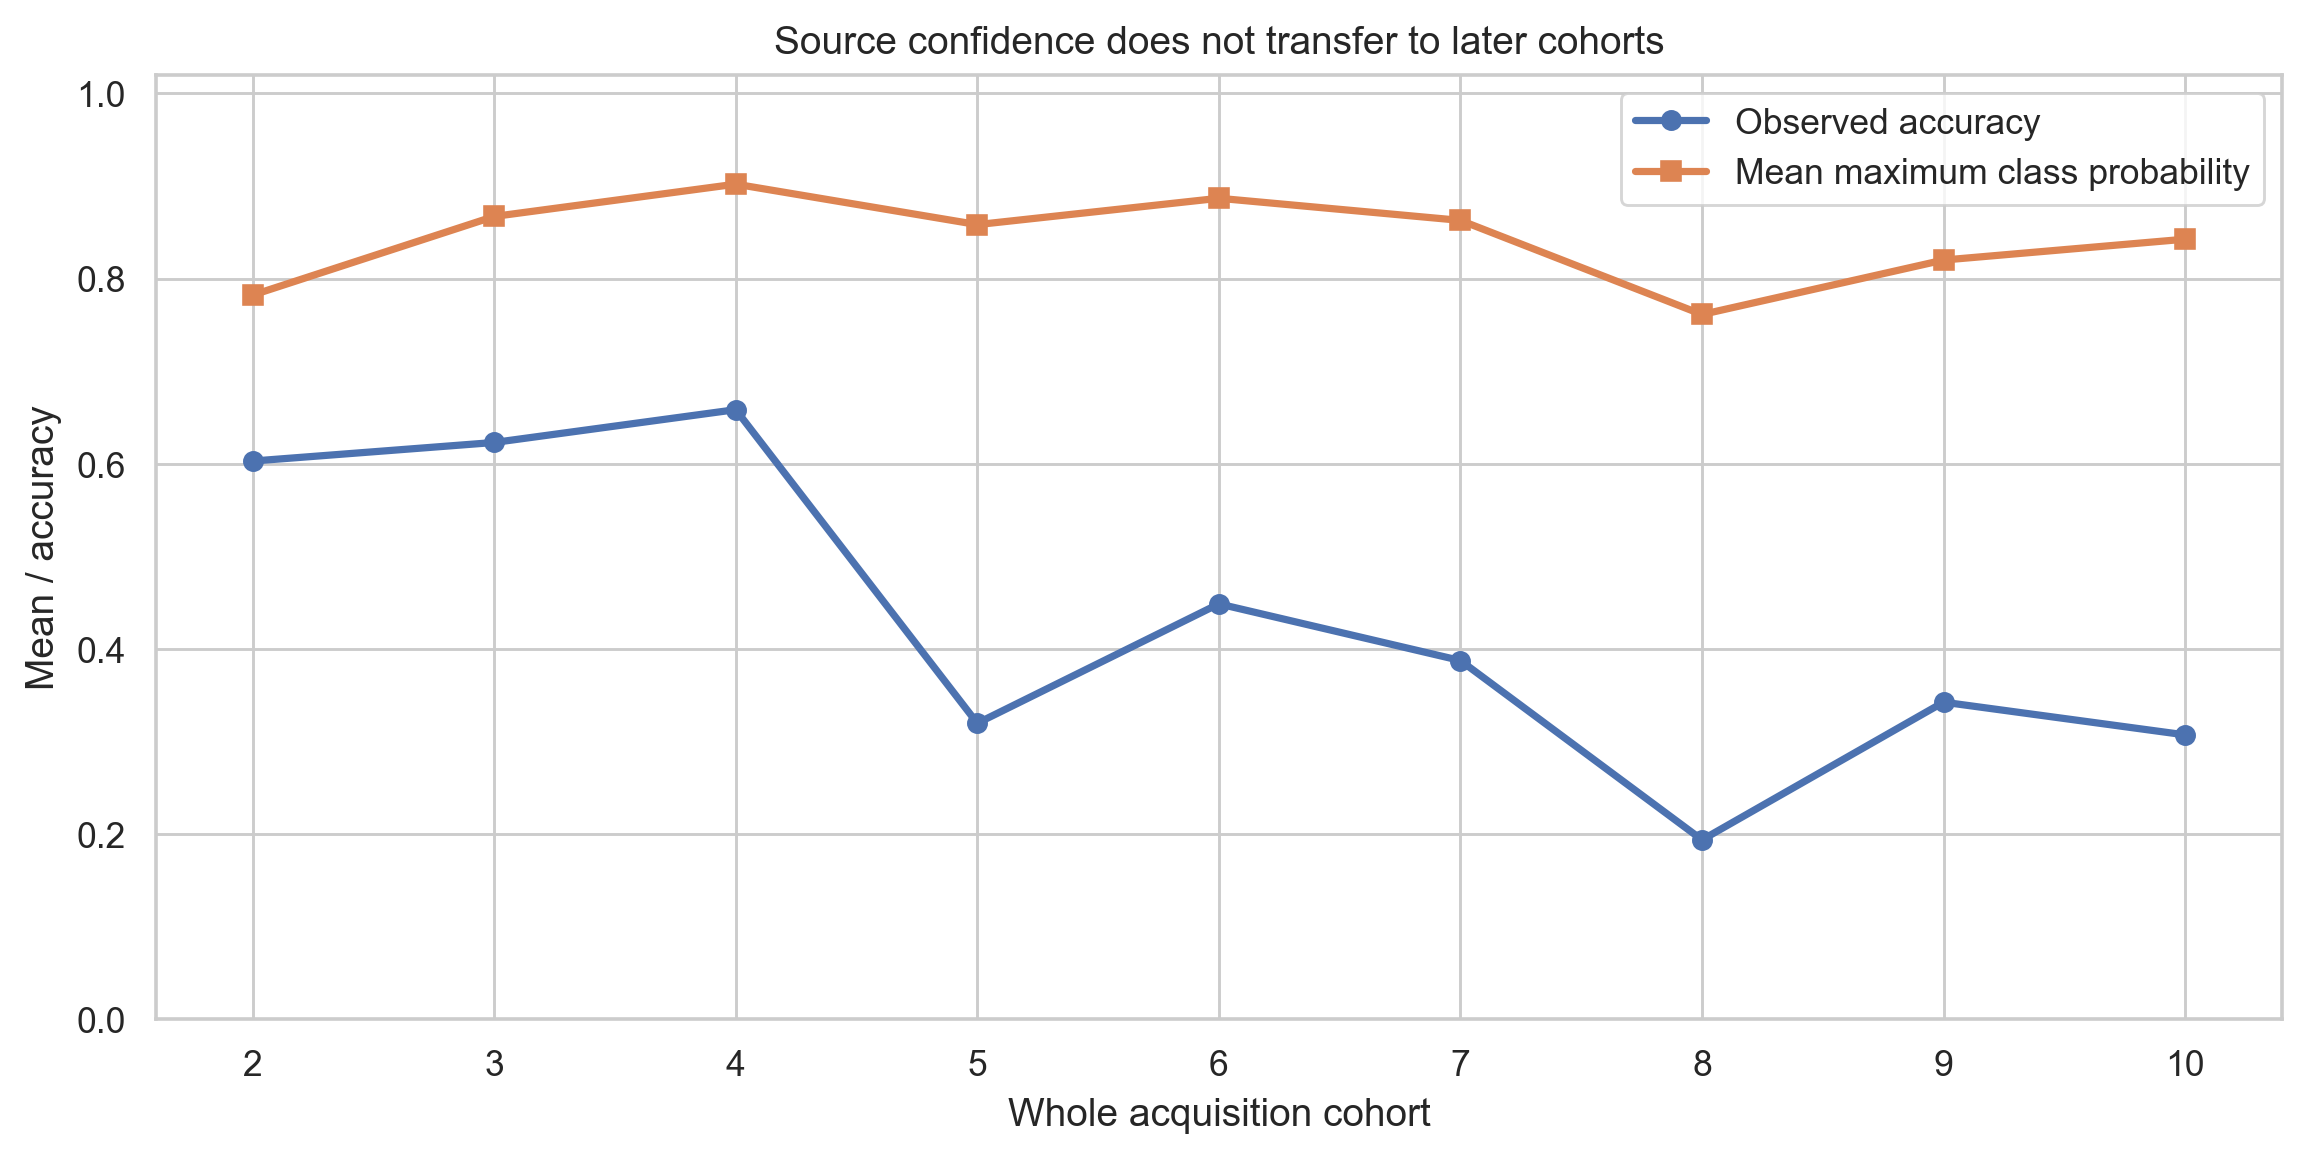
\includegraphics[width=.92\linewidth]{figures/confidence_transfer.png}
\caption{Observed cohort accuracy declines while mean maximum class probability remains high.}
\end{figure}

\section{Day 3 sensitivity}
The 89-row calibration partition scores 87/89 correctly; the separate reference partition scores 84/89. In batches 2-10, mean raw maximum probability exceeds observed correctness by 0.18 to 0.57. Calibration therefore transfers poorly beyond the small source cohort.

For each later cohort, the sensitivity calculation reweights per-class accuracy by batch-1 reference proportions, renormalized over classes present in that cohort. The standardized minus observed accuracy ranges from -0.204 to +0.077; in most cohorts, common-class standardized accuracy also remains poor. The values vary in direction and are not a causal decomposition. Classes absent from a cohort are omitted from the standardized calculation, so it does not recover a six-class counterfactual.

\begin{figure}[h]
\centering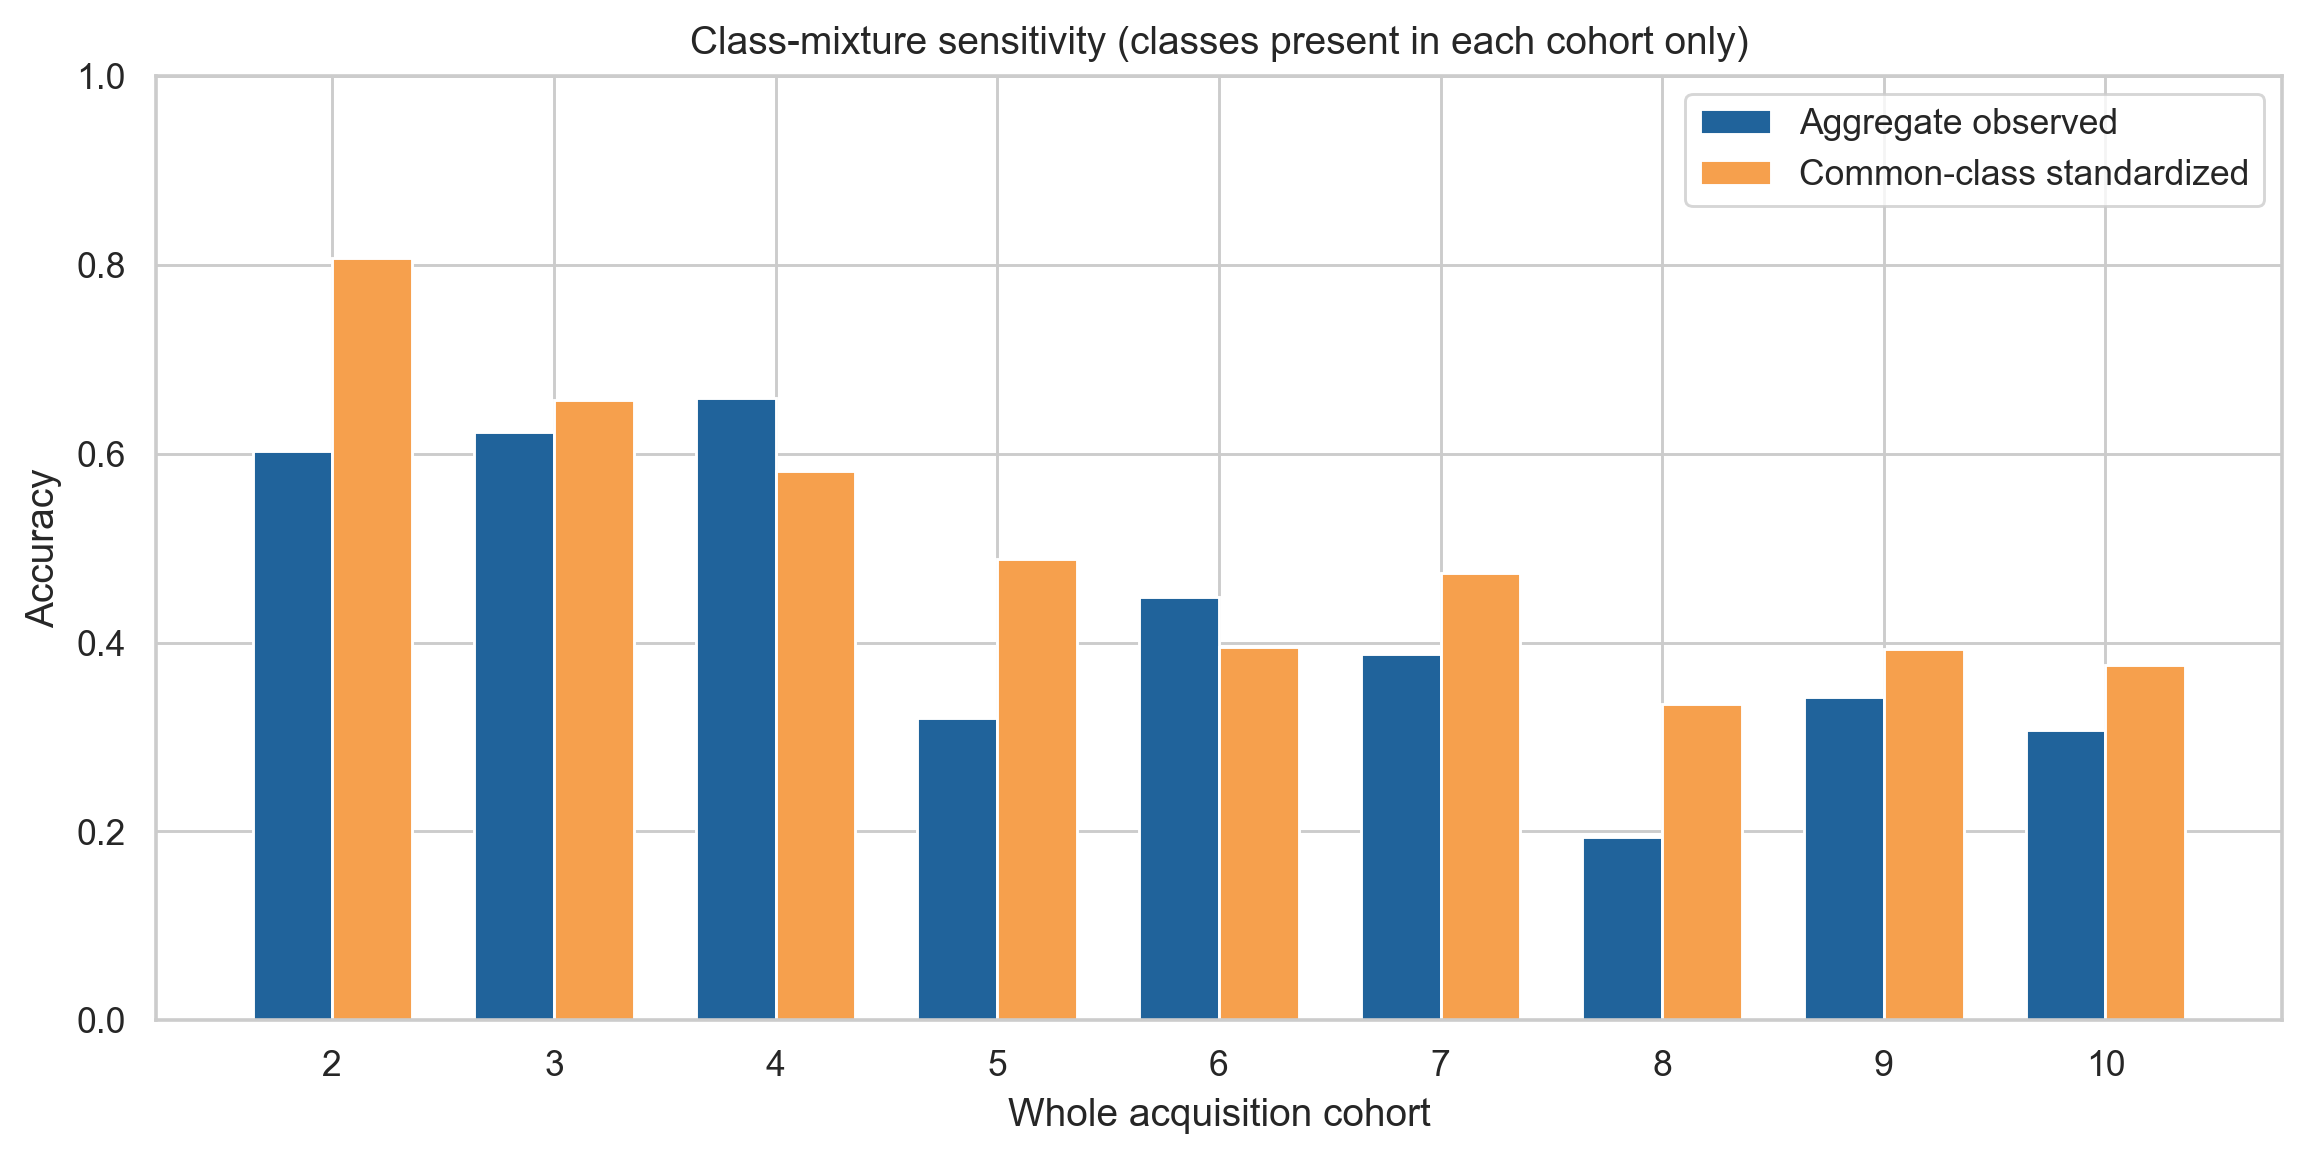
\includegraphics[width=.9\linewidth]{figures/class_mix_sensitivity.png}
\caption{Aggregate accuracy and descriptive common-class standardization. Absent classes are not imputed.}
\end{figure}

The sensitivity supports a narrow interpretation: both within-class degradation and changes in class composition can affect cohort accuracy, while the frozen calibrated correctness channel substantially overstates realized performance. Sensor and class changes remain entangled in this observational dataset; the diagnostic does not assign causal responsibility.

\section{Conclusions and limitations}
The controlled synthetic Phase 3 results remain the evidence for known interventions. The external UCI evidence adds one natural acquisition-cohort case and exposes severe calibration-transfer error. It does not validate population safety, human benefit, causal explanation, or broad external generalization. Historical data are limited to 445 rows from one early batch, test cohorts are unequal, acquisition ordering is coarse, and classes are absent in some batches. Interval assumptions are not met as a guarantee. V2 and adaptation remain separately identified synthetic, outcome-informed extensions.

The submitted Phase 2 DOCX remains the research basis; no instructor feedback was received. Changes documented here are implementation decisions. The original submitted Phase 3 archive and Day 1/Day 2 packages are retained. Reproduction commands, provenance hashes, source, results and limitations accompany this report. The full result is available in the Day 3 archive.

\bibliographystyle{plain}
\bibliography{REFERENCES}
\end{document}
